\documentclass{article}
% \usepackage[utf8]{inputenc}
\usepackage[backend=biber,citestyle=ieee]{biblatex}

\usepackage{pgfgantt}
\usepackage{graphicx}
\usepackage{xcolor}
\usepackage{float}
\usepackage{subfig}

% \usepackage{a4wide} 

\usepackage{fancyhdr}   %sidhuvud
\pagestyle{fancy}

\addbibresource{sources.bib}

\newcommand{\getauthor}{Oscar Fredriksson} %Author
\newcommand{\gettitle}{NS3 - Lab} %Title

\title{\gettitle}
\author{\getauthor}
\date{April 2021}

\begin{document}

    \pagenumbering{gobble}
    \maketitle

    \newpage

    \pagenumbering{arabic}

    \fancyhf{}
    \lhead{\getauthor}
    \rhead{\gettitle}
    \rfoot \thepage

    \section{}

    \subsubsection*{What is the network topology?}
    The simulated network topology is a simple point to point connection, a diagram of the topology can be seen in figure \ref{fig:topology}.

    \begin{figure}[H]
        \centering
        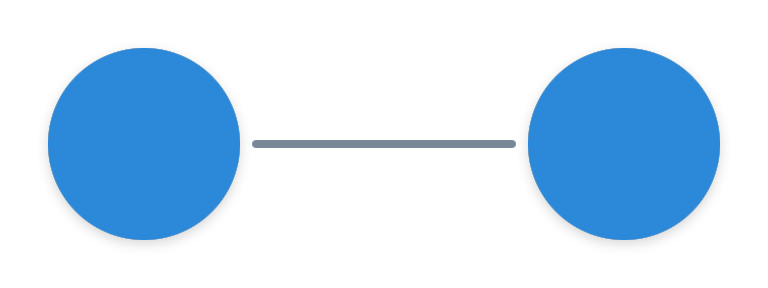
\includegraphics[width=0.5\textwidth]{img/topology.png}
        
        \caption{The simulated topology, a simple point to point connection.}
        \label{fig:topology}
    \end{figure}

    \subsubsection*{How many queues are used in each node? How are they configured?}
    The system uses two different queues, a \verb|FifoQueueDisc| that can hold a specific number of packets configured by the parameter \verb|queueSize| and a \verb|DropTailQueue| that can hold a single packet and drops any overflow. The \verb|FifoQueueDisc| feeds into the \verb|DropTailQueue| which means a total queue size of \verb|queueSize+1| with any extra packets on route to each node gets dropped by the \verb|DropTailQueue|. 

    \subsubsection*{Does the channel introduce errors?}
    

    \subsubsection*{What are the configuration variables of the code?}

    \subsubsection*{What output files are generated?}

    \newpage
    % \printbibliography

\end{document}